% Hadron-Hadron Scatteing
%%%%%-------PROVA-------------
%\documentclass[12pt]{report}
%\usepackage[british]{babel}
%\usepackage{amsmath}
%\usepackage{amsfonts}
%\usepackage{amssymb}
%\usepackage{geometry}
%\geometry{hmargin={2cm,2cm},vmargin={2cm,2cm}}
%\usepackage{caption}
%\captionsetup{format=hang}
%\usepackage{graphicx}
%\usepackage{enumitem}
%\usepackage{float}
%
%
%
%\usepackage[colorlinks=true, linkcolor=blue]{hyperref} %to use autoref
%%%%%-------------------------

%\begin{document}


\chapter{Hadron-Hadron Scattering}
\label{chap:Hadron-HadronScattering}

In a high energy proton-proton collision we can have either soft or hard processes. Most of the time the hard processes are accompanied by soft interaction, occurring along the hadron interaction.
The hard processes are well understood using perturbation theory, meanwhile the soft processes are not so well understood in fact these processes are described by non perturbative QCD. 

\section{QCD factorization theorem}

The factorization theorem was introduced first by Drell and Yan \cite{DRELL1971578}.

The hadron-hadron scattering is describe in terms of partons extending the formalism used for deep inelastic scattering. 
\begin{equation}
\sigma_{AB}=\displaystyle\int dx_a\,dx_b\,f_{a/A}(x_a)\,f_{b/B}(x_b)\,\hat{\sigma}_{ab \rightarrow X}
\label{eq:factorization1}
\end{equation}
Where X is a partonic/leptonic state and $a\,(b)$ a quark or an antiquark in the hadron $A\,(B)$. This is valid in the "scaling" limit:
\begin{equation}
	s\ \longrightarrow\ \infty \qquad\qquad\qquad \frac{M_X}{s}=\text{finite}
\end{equation}
The problem arise from the perturbative corrections from real and virtual gluon emission. This contribution give a logarithmic divergence (spoil the convergence of the perturbative expansion). These dependencies can be absorbed by the parton distribution function (DGLAP equations). This result in the violation of scaling:
\begin{equation}
	f_{a/A}(x_a)\ \longrightarrow\ f_{a/A}(x_a, Q^2)
\end{equation}  
Now the parton distribution function depend on the momentum scale $Q^2$. 

So, we can rewrite the factorization theorem in \eqRef{eq:factorization1} as:
\begin{equation}
	\sigma_{AB}=\displaystyle\int dx_a\,dx_b\,f_{a/A}(x_a,Q^2)\,f_{b/B}(x_b,Q^2)\,\hat{\sigma}_{ab \rightarrow X}
\label{eq:factorization2}
\end{equation}

Now the \emph{finite} corrections in the perturbative expansion are specific for each process (not universal). This leads in the \eqRef{eq:factorization2} to the $\alpha_s$ series:
\begin{equation}
	\sigma_{AB}=\displaystyle\int dx_a\,dx_b\,f_{a/A}(x_a,\mu_F^2)\,f_{b/B}(x_b,\mu_F^2)\,\left[\hat{\sigma}_0+\alpha_s(\mu_R^2)\hat{\sigma}_1+\dots\right]
\label{eq:factorization3}
\end{equation}
In \eqRef{eq:factorization3} two scales enter the formula:
\begin{itemize}
	\item[--] The \textit{factorization scale} $\mu_F$: this scale separates long- and short- distance.
	\item[--] The \textit{renormalization scale} $\mu_R$: the scale at which is evaluated the strong coupling $\alpha_s$.  
\end{itemize}

The higher-order corrections eliminate the cross section prediction dependencies on $\mu_R$ and $\mu_F$.
Typically, the scales are assumed to be equal.
For example in the Drell-Yan process the standard choice is $\mu_F=\mu_R=M$, with $M$ the lepton pair mass \cite{Campbell2006}. Other cases are the invariant masses of $Z$-boson and top quark or the jet transverse energy to study \cite{Campbell2006} the production cross sections for Z-bosons, top quarks and large E T jets.

The parton distribution functions used in the hard scattering are solution of the DGLAP (Dokshitzer–Gribov–Lipatov–Altarelli–Parisi) equation \cite{Lipatov:400357, Gribov:427157, ALTARELLI1977298, Dokshitzer:1977sg}

\begin{equation}
	\mu_F^2\frac{\partial f_{i/H}(x,\mu_F^2)}{\partial\mu_F^2}=\displaystyle\sum_j\frac{\alpha_s(\mu_F^2)}{2\pi}\displaystyle\int_x^1 \frac{dz}{z}\, P_{i\,\rightarrow\,j}(z)\ f_{j/p}\left(\frac{x}{z},\mu_F^2\right)
\end{equation}

Where $P_{i\,\rightarrow\,j}$ are the splitting functions: they are the probability to have a parton of type $i$ that became, by the emission of a quark or a gluon, a parton $j$, carrying fraction $z$ of the momentum of $i$.

The splitting functions have perturbative expansions: 
\begin{equation}
	P_{i\,\rightarrow\,j}(x,\alpha_s)=P_{i\,\rightarrow\,j}^{(0)}(x)+\frac{\alpha_s}{2\pi}P_{i\,\rightarrow\,j}^{(1)}(x)+\dots
\end{equation}

This procedure has been used to calculate Standard Model cross section in $p\overline{p}$ and $pp$ scattering respectively at Tevatron and LHC energies as shown in \figRef{figure:StandardModelCrossSections}.

\begin{figure}[!ht]
	\centering 
	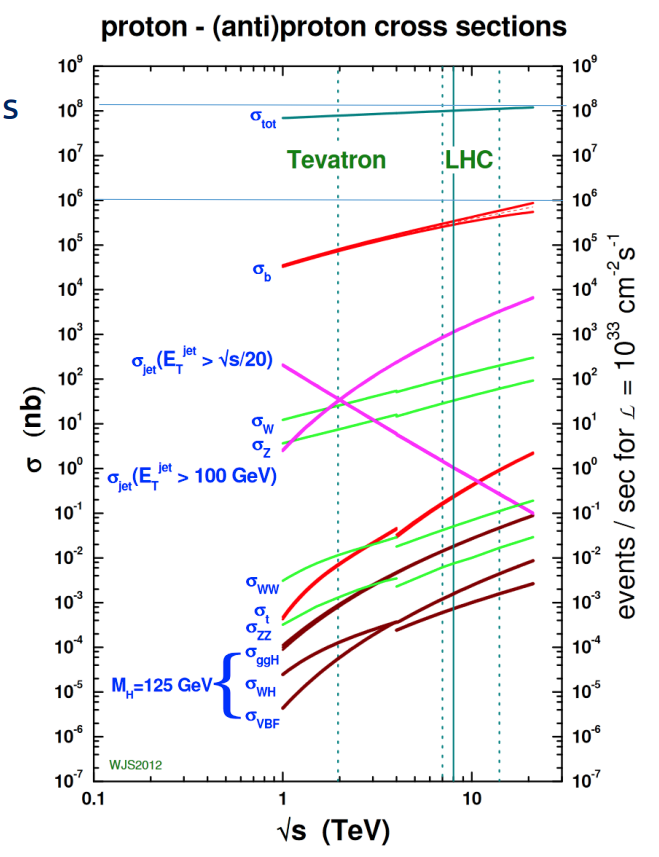
\includegraphics[width=12cm]{img/StandardModelCrossSections_color.png}
	\caption{Next-to-leading order cross sections at Tevatron and LHC colliders energies (the splitting are at the transition between $p\overline{p}$ and $pp$ cross section). Figure from \cite{StirlingPrivate}}
	\label{figure:StandardModelCrossSections}
\end{figure}

The parton distribution functions dependence on $Q^2$ can be derived theoretically via the DGLAP equations. While, the $x$ dependence is given fitting the deep-inelastic and other hard-scattering processes experimental data.
The experimental coverage in $(x,Q^2)$-plane is shown in \figRef{figure:xQ2planeCoverage} 
where is also underlined the relationship between $(x,Q^2)$ and kinematic variables in Drell-Yan processes for a final state with invariant mass $M$ and rapidity $y$ is shown, further details in section 2 of \cite{Campbell2006}. Assuming that the factorization scale $Q$ is equal to $M$ (The reference center of mass energy is $13\ \mathrm{TeV}$). So, for two incoming particles with four-momentum respectively $p_1$ and $p_2$ the relations with $y$ and $M$ are:  
\begin{equation}
	\begin{aligned}
		&p_1^\mu=\frac{\sqrt{s}}{2}(x_1,0,0,x_1)\\
&p_2^\mu=\frac{\sqrt{s}}{2}(x_2,0,0,-x_2)
	\end{aligned} \quad\Longrightarrow\quad x_1=\frac{M}{\sqrt{s}}e^y\qquad x_2=\frac{M}{\sqrt{s}}e^{-y}
\end{equation}
where  $s=(p_1^\mu+p_2^\mu)^2$.


\begin{figure}[!ht]
	\centering 	
	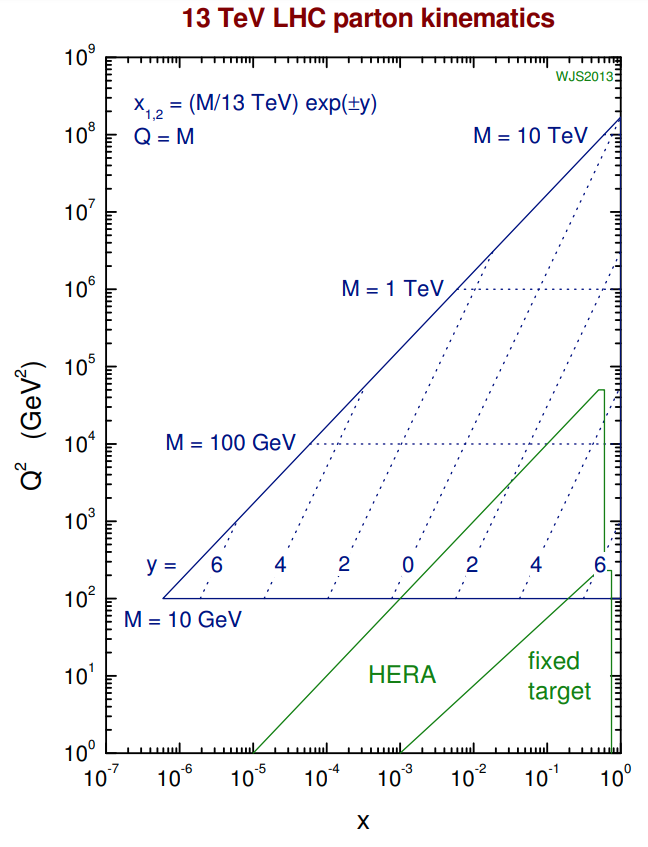
\includegraphics[width=12cm]{img/xQ2planeCoverage.png}
	\caption{Graphical representation of the parton $(x,Q^2)$ variables coverage of different experiments. For LHC these $x$ and $Q^2$ are related to the kinematic variables $y$ and $M$. Figure from \cite{StirlingPrivate}}
		\label{figure:xQ2planeCoverage}
\end{figure}

\section{Partonic cross section}

Partonic cross section is one of the fundamental ingredients in our recipe. This can be calculated in a perturbative series in $\alpha_s$ from QCD first principles using quantum field theory.

The calculation at the leading order (LO) is performed evaluating all the possible tree-level Feynman diagrams for every process. Evaluating the squared matrix element and integrating over the available phase space (analytically or numerically).

Already here, we can encounter some divergence that have to be avoided imposing restriction on the phase space.

\subsection{Higher order calculations}

The LO calculation can describe broad feature of a particular process and provide a first estimation of its cross section but in many cases this is insufficient.

The main source of uncertainty derives from the LO dependence  on the unphysical renormalization and factorization scales. Some process may contribute only when going beyond the first approximation, and some divergence can be resummed. 

To the next-to-leading orer (NLO) calculation participate all the Feynman diagrams that take an extra $\alpha_s$. This contribution can arise in two different way:
\begin{itemize}
	\item Virtual: internal lines (loops);
	\item Real: external lines (real particles).
\end{itemize}

Virtual corrections contains infrared divergences, arising from the integral on the loop circulating momentum, that cancel against infrared singularities given by collinear emissions or soft emissions \cite{PhysRevBloch, KinoshitaToichiro, PhysRevLee}. 

A common strategy for the rinormalization is dimensional regularization: consists into perform the calculation in a $D=4-2\epsilon$-dimensional space ($\epsilon<0$), in that way the singularities appear as single and double poles in $\epsilon$. Than, the limit $\epsilon\rightarrow0$ is taken after the divergences have cancelled.

This NLO calculation with regularization allows to extend the treatment to zero transverse momentum.

The importance of higher order calculations can be seen with the following example. In a $Z$ boson production:
\begin{enumerate}[label=$\arabic*)$]
	\item \textbf{LO}: the $Z$ is produced without transverse momentum ($p_T$), anything can recoil against the $Z$ for momentum conservation.
	\item \textbf{NLO}: the $Z$ acquire a finite $p_T$, in this case the $Z$ boson $p_T$ is balanced by a single \mbox{parton/gluon}.
	\item  \textbf{NNLO}: the $Z$ $p_T$ can be balanced by two jets. 
\end{enumerate}



Another important benefit of performing a NLO calculation is the the reduction of the dependence on the unphysical renormalization ($\mu_R$) and factorization ($\mu_F$) scales.
It is proven that higher order calculations is that observables calculated to order $\alpha_s^{\,n}$ are dependent on the unphysical scales only at order higher than $\alpha_s^{\,n+1}$ \cite{Campbell2006}. The range of predictions corresponding to different scale choices is usually attributed to \textit{theoretical uncertainties}.

\section{Parton Showers}

A different approach, instead than calculating order by order in the perturbative expansion, is to use an \textit{all-order} approach in order to describe the phenomena observed at high-energy colliders. 

different all-order approaches exist e.g. resummation and parton showers. Resummation is based on the observation that in many quantities the smallness of the expansion coefficients $\alpha_s$ is violated by large logarithmic enhancements. This take the dominant contribution from each order and "resum" them by means of an evolution equation. 
The main problem in QCD is related to the fact that lot of quantities have correction of the form $\alpha_s^n\log^k(Q_i/Q_j)$ where $Q_i$ and $Q_f$ are two different energies scales, for example:
\begin{itemize}
	\item[--] Renormalization and factorization scales logs: $\alpha_s^n\log^n(Q^2/\mu_f)$
\end{itemize}
Various methods to perform this resummation exist.

%%%% GRAPH on pT Z with effect of resummation 
An example is the $Z$ production $p_T$ spectrum shown in \figRef{figure:pT_Z_CDF}. A comparison between experimental CDF data and theoretical predictions is shown: in the low $p_T$ region the \textit{all-order} approach regularize the divergence of the fixed order calculation and describe the data better then the last one. 

\begin{figure}[!ht]
	\centering
	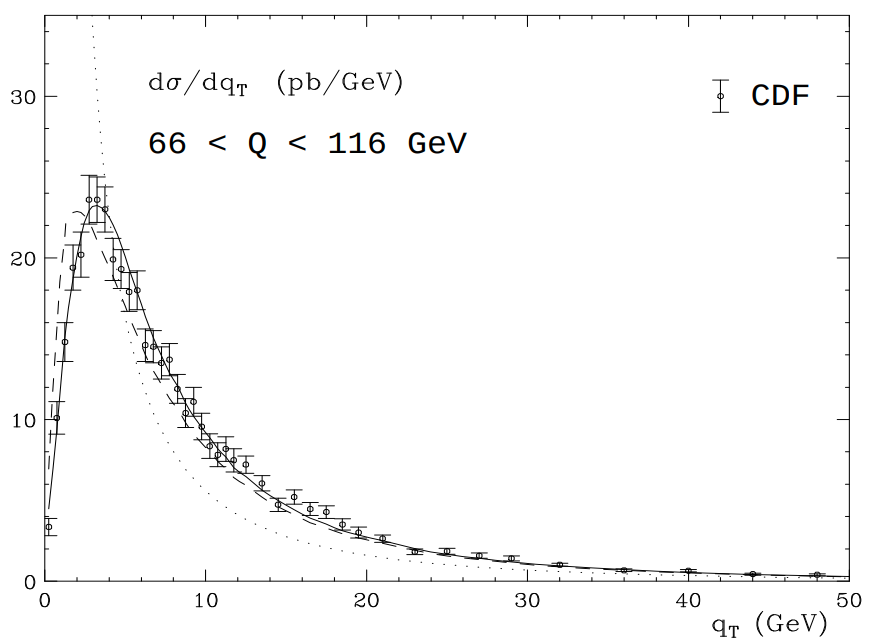
\includegraphics[width=12cm]{{img/pT_Z_CDF.png}}
	\caption{CDF data on $Z$ production cross section at Tevatron collider, CDF experiment, the predictions from fixed order calculation (dotted) with resummation (dashed), and with the inclusion of power corrections (solid) are compared. Figure take from \cite{kulesza2002electroweak}}
	\label{figure:pT_Z_CDF}
\end{figure}

An other \textit{all-order} approach is parton showers, this is implemented in different programs  \textsc{pythia} \cite{PYTHIA2015}, \textsc{herwig} \cite{Herwig2008} and \textsc{sherpa} \cite{SHERPA2004}. This start from few parton arising from hard interaction and than these are related to partons to a lower energy scale close to $\Lambda_{QCD}$ using the DGLAP evolution equation formalism, the solution at this equation can be write using a Sudakov form factor arising from the probability of no gluon emission in the evolution from higher scale to lower scale.



In the parton showering process, additionally to the kinematic variable (momentum fraction $z$ and an azimuthal angle $\phi$) and flavours of the partons, an evolution variable $t$ is generated.\textsc{Pythia8} use as  evolution variable the squared of the relative transverse momentum of the two partons in the splitting ($p_T^2$). Different choices are made in \textsc{herwig} and \textsc{sherpa}.

So as mentioned before, the shower evolution is based on the standard (LO) DGLAP splitting kernels P(z)
\begin{align}
P_{q\,\rightarrow\,qg}(z) & = C_F\frac{1+z^2}{1-z} \\
P_{g\,\rightarrow\,gg}(z) & = C_A\frac{(1-z(1-z))^2}{z(1-z)} \\
P_{q\,\rightarrow\,q\overline{q}}(z) & = T_R(z^2+(1-z)^2)
\end{align} 
where $C_F=\frac{4}{3}$, $C_A=N_C=3$ and $T_R=\frac{1}{2}$ multiplied by $N_f$ if summing over all contributing quark flavours.

Both Initial State Radiation (ISR) and Final State Radiation (FSR) algorithms are based on these splitting kernels.

The probabilities of emitting radiation as one moves in the decreasing evolution variable sequence are:
\begin{align}
	FSR: \qquad\quad & \frac{d\mathcal{P}_{FSR}}{dp_T^2} = \frac{1}{p_T^2}\displaystyle\int \frac{dz}{z}\,\frac{\alpha_s}{2\pi}P(z)\label{eq:FSR1}\\
	ISR: \qquad\quad & \frac{d\mathcal{P}_{ISR}}{dp_T^2} = \frac{1}{p_T^2}\displaystyle\int \frac{dz}{z}\,\frac{\alpha_s}{2\pi}P(z)\,\frac{f'(x/z,p_T^2)}{f(x,p_T^2)}\label{eq:ISR1}
\end{align}

We can write our Sudakov form factor as:
\begin{equation}
	\Delta(p_T^2)=\exp\left( -\displaystyle\int_{p_T0}^{p_T'} \frac{d\mathcal{P}_{PS}}{dp_T^2} \,dp_T\right) \qquad\text{ with } \quad PS=ISR,\ FSR
	\label{eq:sudakovFormFactor}
\end{equation}

So, the Sudakov form factor give the probability of a parton to evolve from an harder scale to a softer scale without emitting a parton harder than some resolution scale. 

The introduction of the Sudakov form factor resums all the effects from the soft and collinear gluon emission. For more details and some plots of different Sudakov form factor values see section 3.5 of \cite{Campbell2006}.

\subsection{Merging parton showers and matrix element calculations}

So, regions dominated by soft and collinear gluon emission are described very well by parton showers approach, on the other hand regions where partons are  energetic and widely separated are well described by matrix element calculations. 

The best approach would be to combine the two different description, This require an universal formalism for parton showers and matrix element calculations. This was created in 2001 and it is call "Les Houches Accord" \cite{LesHouchesAccord}.
In order to combine the two approach some care must be taken: there is the risk of double counting. There are different technique that prevent this risk for example CKKW \cite{CKKW2001}.

A more best way is to combine NLO matrix element calculation with parton showers this is done by Frixione, Nason, Webber in the \textsc{mc@nlo} framework \cite{FxFx1,FxFx2,FxFx3}. In this scenario  the double counting is given by the fact that at NLO one emission is made real and the progress of the parton shower give a double counting between real and virtual emission as shown in \figRef{fig:DoubleCounting}


%%%
%%% Immagine di Frixi.. presentation
\begin{figure}[H]
	\centering
	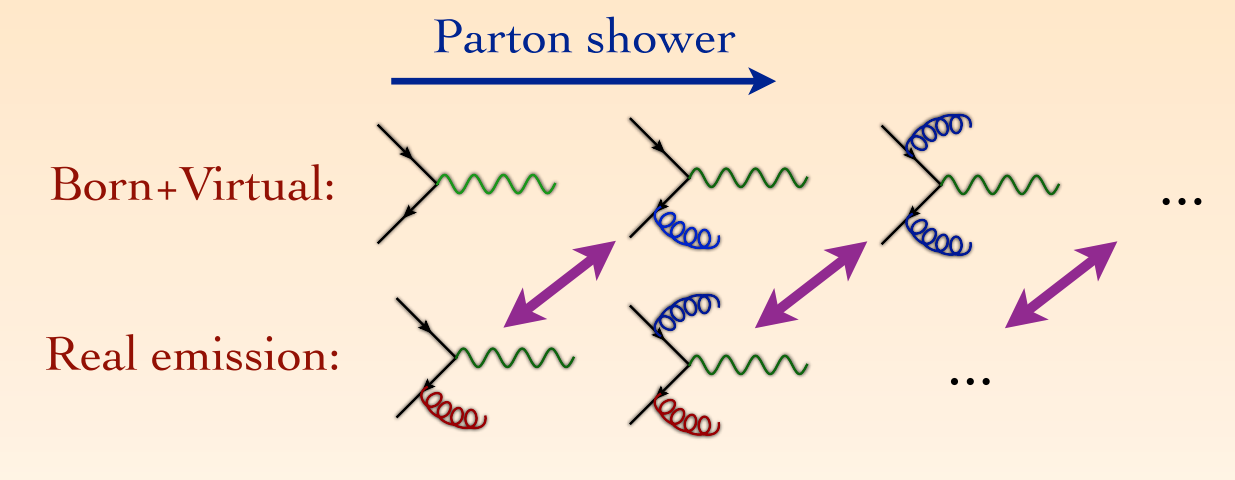
\includegraphics[width=12cm]{{img/DoubleCounting.png}}
	\caption{See https://indico.cern.ch/event/221788/attachments/361954/503905/frederix.pdf}
	\label{fig:DoubleCounting}
\end{figure}
%%%


\section{Parton distribution functions}

The information on the quark distribution inside an hadron $f_{q/p}(x,Q^2)$ arise from lepton-hadron DIS experiments and from lepton-pair production in hadron-hadron collisions (Drell-Yan processes) and jet measurements to study gluon distribution $f_{g/p}(x,Q^2)$. All these quantities are the experimental input in order to evaluate the PDF inside the hadron while the $Q$ evolution can be described by DGLAP equation.
The evolution of the PDF can be run either with a NLO calculation or with a NNLO calculation.

The kinematic region covered by experiments was shown in \figRef{figure:xQ2planeCoverage}. At very low x and $Q^2$ the DGLAP evolution is believed to be no longer applicable and a BFKL [ADD citations from \cite{Campbell2006} page 44] description must be used, but there are no evidence of this so the DGLAP approach is use as default in all the PDF analysis.

A lot of process are available for the PDFs evaluation and a lot of PDF set have been generated for example \figRef{fig:NNPDF31} shown the NNPDF3.1 set \cite{NNPDF3.1} at NNLO for a virtuality $Q^2=10\ \mathrm{GeV^2}$ (left) and $Q^2=10^4\ \mathrm{GeV^2}$ (right). 

\begin{figure}[!ht]
	\centering
	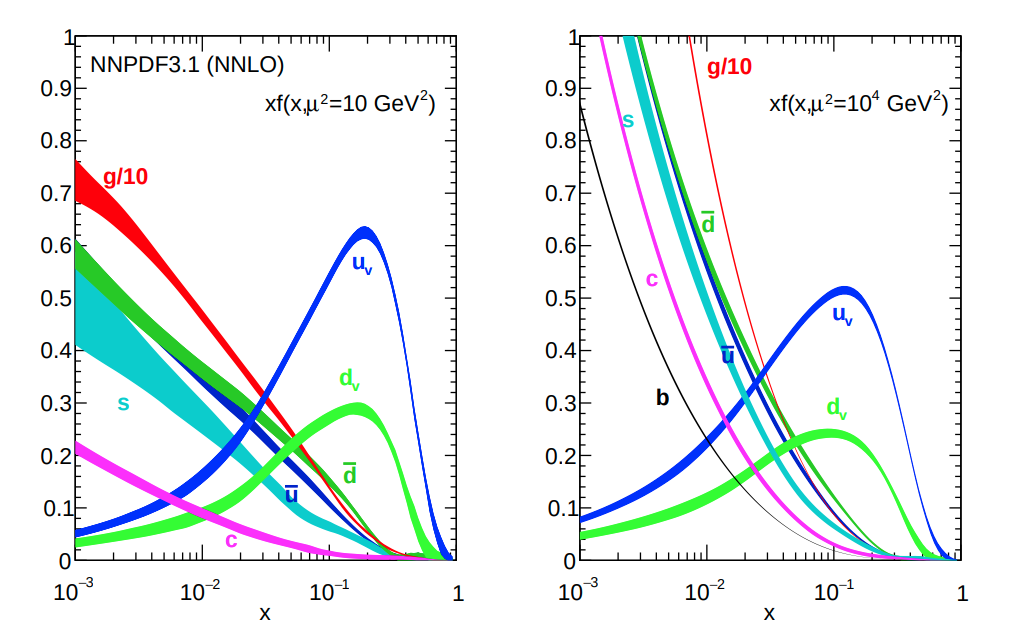
\includegraphics[width=12cm]{{img/NNPDF3.1.png}}
	\caption{The NNPDF3.1 NNLO PDFs, evaluated at $Q^2 = 10\ \mathrm{GeV}^2$
(left) and $Q^2=10^4\ \mathrm{GeV}^2$ (right). At low $x$ the contribution from the gluon in the dominating one while at higher x the dominant contribution is from the valence quarks. The PDF $Q$ evolution shows that when our proton is probed to higher $Q^2$ the resolution increase (higher $Q$ correspond to smaller distance resolution) and so we have a bigger contribution from the sea quarks at low $x$ values.}
	\label{fig:NNPDF31}
\end{figure}

Note that the gluon contribution have been scaled of a factor 10 in fact in the low $x$ region, $x<0.01$, the gluon contribution is the dominating one. While, at high $x$ value the valence quarks dominate the PDF. In \figRef{fig:NNPDF31} we can also see that with increasing virtuality ($Q^2$) at low x the density of the sea quarks increase this is related to the fact that our hadrons are probed at higher energy and the probe resolution is proportional to the energy. 
\begin{equation}
	\text{Resolution}\sim\frac{\hbar}{Q^2}
\end{equation}
So, when probed at higher energy the hadron appears denser than when are probed at lower energy. This, as will be discussed in the next chapter, is related to the higher number of interaction between partons in a single hadron-hadron collision. The phenomenon of having more than one interaction between partons in a single hadron-hadron collision is called multiple parton interaction and we want to introduce this concept in the next chapter.


\section{A real proton-proton collision}

We have understood that the complexity in the description of a proton-proton collision arise from composite nature of the protons. In this chapter we discussed the importance of the QCD factorization theorem that help us in the calculation of the hadronic cross section with the convolution between the partonic cross section and the PDF. We have discussed the importance of the parton shower algorithm were a set of partons are evolved in a more complex final state by emissions in the initial and final states.

All these processes are important in the description of a real proton-proton collision but also the partons that are left unscattered are non-color singlet and contribute to the complex final state observed in the experiment, and additionally, as mentioned before, nothing prevent additional partons scatterings from taking place and growing more and more the complexity of the partons final state. 

Than, another problem is related to the not-well-understood hadronization process.
Hadronization is not known from first principles and different models are implemented in different programs: the \textit{cluster fragmentation model} implemented in \textsc{herwig} and the \textit{string fragmentation model} in \textsc{pythia} simulated this process of hadronization where the set of final-state partons are transformed into a set of hadrons. All these processes are shown schematically in \figRef{fig:Processes}.

\begin{figure}[!ht]
	\centering
	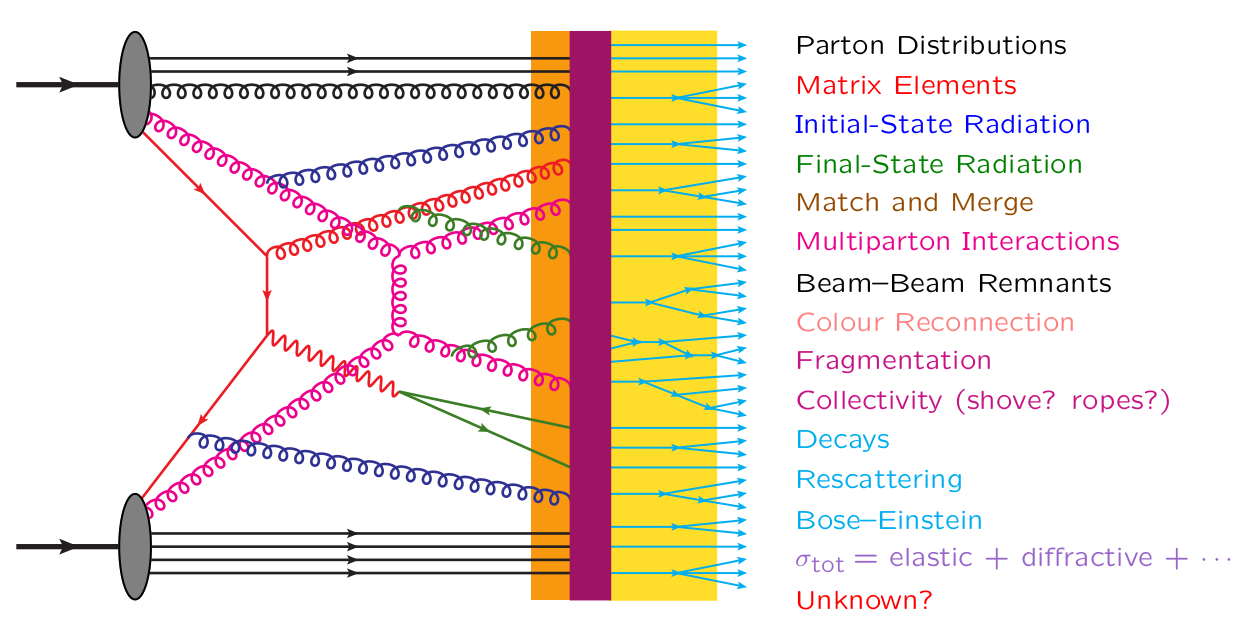
\includegraphics[width=0.98\textwidth]{{img/Processes.png}}
	\caption{A schematic representation for a $pp$ collision. Reading the image from left to right one can have an idea on the evolution of the system. The two incoming hadrons enter the scattering from the left side, the read line indicate the main hard scattering and the fuchsia one the second parton scattering (MPI) each interaction is associated with initial (blue) and final (green) state radiation, the unscattered partons (black lines) re-enter the color reconnection and hadronization processes. Than the new formed hadrons (lightblue) can undergo to different decays.}
	\label{fig:Processes}
\end{figure}

Next chapter describe the \textsc{pythia} Monte Carlo generator in more details. \textsc{pythia} introduce different free parameter that need to be tuned with experimental data from Tevatron and LHC. The tune methods are described in \chapRef{chap:TuneprocedureCP5TuneandMCNNTUNES}



%%% ---



%In a \textbf{proton-proton collision}, additionally to the main hard scattering that can be described performing Matrix Element calculations (MEs) , also other scattering processes are possible. To well understood the proton-proton collision we need to describe other processes, besides to the hard scattering, that can underlying to this  \textbf{Multi Parton Interaction} (MPI) and the \textbf{Beam-Beam Remnants} (BBR).




%\end{document}